
\chapter{Simulation of Tele-operation}
\label{c6_simulation}
In this chapter, simulation of a tele-operated mobile robot is presented. In tele-operation, the human operator observes a remote scene through camera(s), and manipulates the local steering wheel and accelerator pedal, as illustrated in Figure \ref{fig:teleoperation} . The command is transmitted to the mobile robot over wireless network. The operator's response is based on the latest feedback images from the cameras. In general, there is a time lag when communication takes place over wireless network. The time lag deteriorates the human performance as discussed in \cite{chen2007human} and references therein.  This chapter simulates the tele-operation both without and with time delay in transmission network.
\begin{figure}
	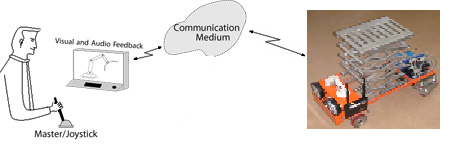
\includegraphics[width=\linewidth,keepaspectratio]{Chapter6/fig/teleoperation}
	\captionof{figure}{Teleoperation  architecture }
	\label{fig:teleoperation} 
\end{figure}

\section{Modeling of Mobile Robot}
The standard kinematic model, as described in \cite{campion1996structural}, of the mobile robot was used for the simulation. The use of kinematic model is justified as  the vehicle is expected to move at relatively slow speed and model is simple. Inputs to the model are left and right rear wheel velocities. The front wheels are steered to satisfy the Ackerman condition, as presented in Chapter \ref{ch_3:Design}  and are assumed to attain the desired angle instantaneously. Therefore, the robot can be treated as differential drive robot.  The kinematic model of the platform is presented below:

\begin{equation}
\label{eqn:KinematicModelOfRobot}
\begin{pmatrix}
\dot{x}\\ 
\dot{y}\\ 
\dot{\theta}
\end{pmatrix}
=
\begin{pmatrix}
\cos \theta & 0 \\
\sin \theta & 0 \\
0& 1
\end{pmatrix}
\begin{pmatrix}
r_w/2 & r_w/2\\
r_w/ l & -r_w/l
\end{pmatrix}
\begin{pmatrix}
\dot{\phi_L}\\
\dot{\phi_R}
\end{pmatrix}
\end{equation}


where ,  $l$ is the distance between the rear wheels, $r_w$ wheel radius. $\dot{\phi_R}$ and $\dot{\phi_L} $ are the rotational velocities of left and right wheels. 
The operator station sends the command $u_1$ and $u_2$ over the wireless network. In general, it will be delayed by time $\delta$. These commands are interpreted by the robot controller as the left and right wheel velocities.  Therefore, by taking the time delay into consideration one can write
\begin{equation}
\begin{pmatrix}
\dot{\phi_R}(t) \\
 \dot{\phi_L}(t)
\end{pmatrix}
=
\begin{pmatrix}
u_r(t-\delta)\\
u_l(t-\delta)
\end{pmatrix}
\end{equation}

The control inputs to the mobile robot  $u_r$ and $u_l$ are generated by the operator based on the visual data available to the person. Hence, a model of the human operator needs to be used for the simulation of the complete loop.


\section{Model of Human Operator}
In order to simulate the tele-operation loop, one needs a mathematical model of a human operator. The mathematical  model of the operator's action is approached assuming a car driving metaphor.
 The video feedback, which the operator receives of the remote environment, give him the idea of the vehicle's  position and the tentative next goal point (p) based on a lookahead distance (l). He then constructs a  virtual path mentally and tries to manoeuvre or steers the robot to follow that path as shown in Figure \ref{fig:drivingStratagy}. As he moves forward the goal point keeps changing until he reaches the desired location. This methodology of path tracing is known as pure pursuit \cite{coulter1992implementation}. 
\begin{figure}
	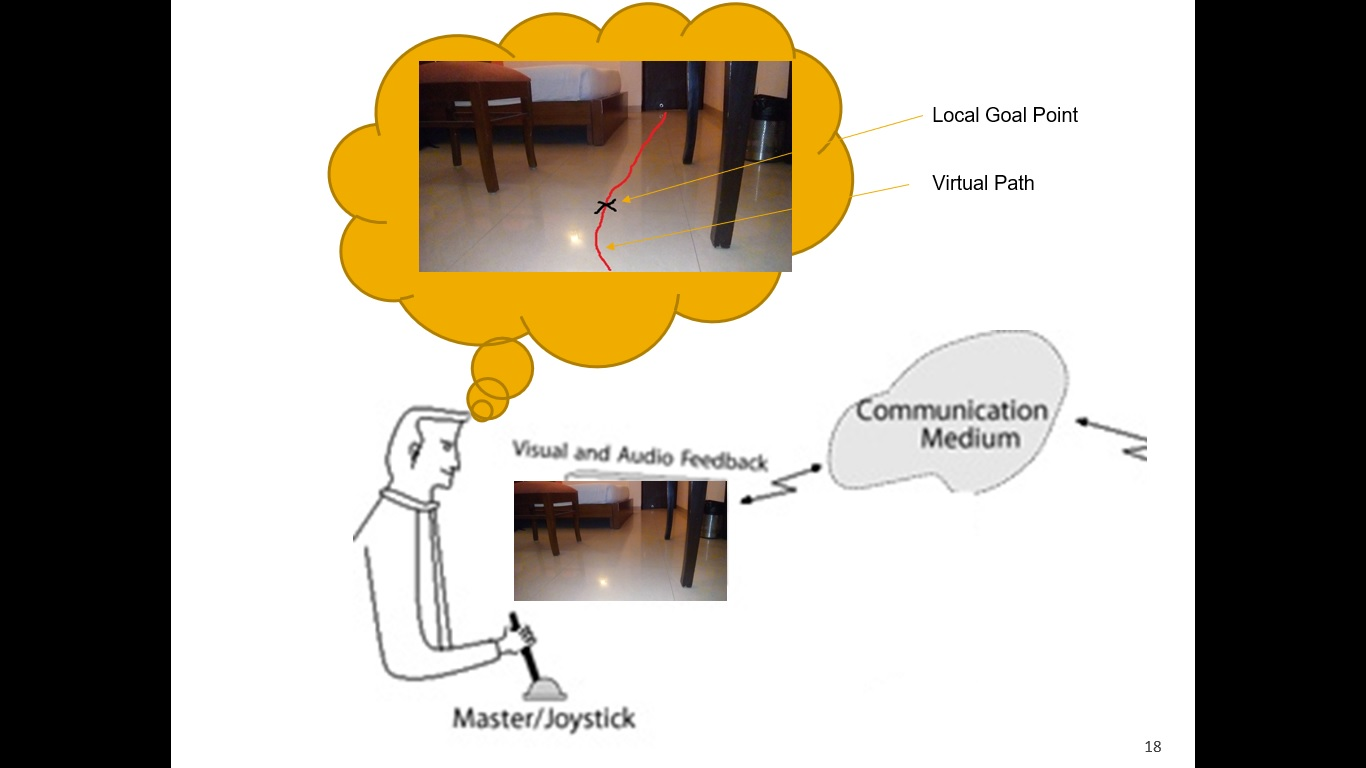
\includegraphics[width=\linewidth,keepaspectratio]{Chapter6/fig/mentalMap}
	\captionof{figure}{Assumed driving strategy  }
	\label{fig:drivingStratagy} 
\end{figure}

The mathematical model for the pure pursuit method of path following can be derived as given in Figure \ref{fig:purePGeo}.
As shown in Figure \ref{fig:purePGeo}, the origin of the coordinate system is at point $o$, the middle of rear axis of the robot. As the differential drive robot  can move only about a circle with center  lying on the line along its rear axis. An arc $OP$ of radius $r$, is drawn with center $O_1$ and passing through $o$ and $p$. Where $p$ is a point on the path to be traced by the robot. The linear distance  between the points $o$ and  $p$ is called the\textit{ look ahead distance} $l$. This distance in the case of a tele-operated robot will depend on the field of view of camera at the remote location and the obstacles present in the remote environment.

If $(x,y)$ is the coordinate of point $p$ in $X-Y$ coordinate system, then 
\begin{equation}
x^2+y^2=l^2, \quad \quad d=r-x
\end{equation}

Similarly, from triangle $p, x, o1$ we get
\begin{equation}
d^2+y^2=r^2\quad \Rightarrow (r-x)^2+y^2=r^2 \quad \Rightarrow x^2+y^2-2rx=0
\end{equation}
Replacing $x^2$ and $y^2$ in Equation 6.4 with Equation 6.3, we get
\begin{equation}
\label{ppControl}
2rx=l^2\quad \quad \Rightarrow r=\frac{l^2}{2x}
\end{equation}
\begin{figure}
	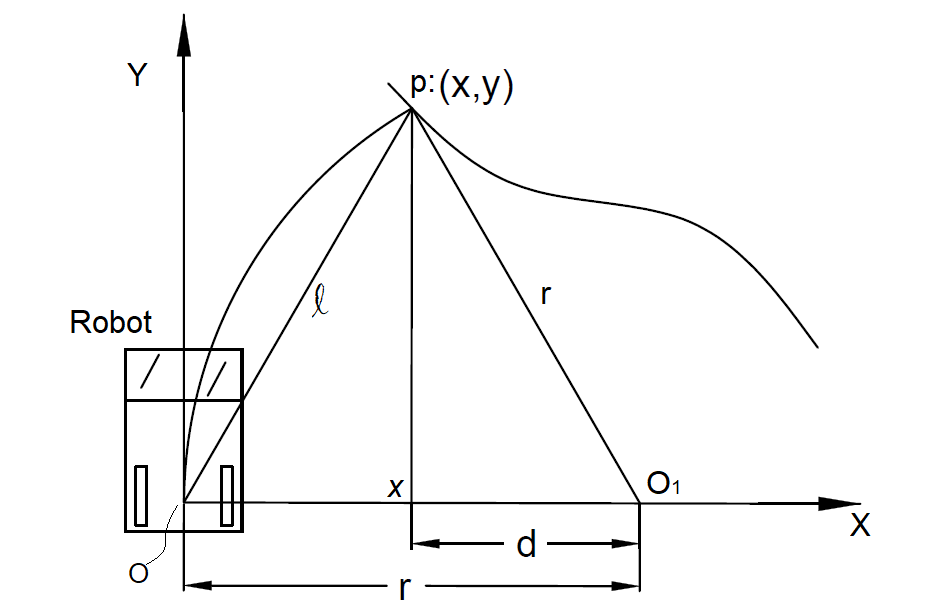
\includegraphics[width=\linewidth,keepaspectratio]{Chapter6/fig/purepesuitgeometry2}
	\captionof{figure}{Geometry of Pure pursuit }
	\label{fig:purePGeo} 
\end{figure}

Once the radius $r$, the desired  linear velocity of the robot $v$ are known, the angular velocity of the vehicle is $\dot{\theta}=-v/r$. The rear wheel  $\dot{\phi}_L(t)$ and $\dot{\phi}_R(t)$ can be calculated from Equation 6.1. Where $\dot{y}=v$ and $\dot{x}=0$. To match the orientation of the vehicle with that in  Figure \ref{fig:purePGeo}, $\theta=90^o$. We then get

\begin{equation}
\begin{pmatrix}
\dot{x}\\
\dot{y}\\
\dot{\theta}
\end{pmatrix}
=
\begin{pmatrix}
0 & 0 \\
r_w/2 & r_w/2 \\
r_w/l & -r_w/l
\end{pmatrix}
\begin{pmatrix}
\dot{\phi_L}\\
\dot{\phi_R}
\end{pmatrix}
\quad \Rightarrow 
\begin{pmatrix}
\dot{\phi_L}\\
\dot{\phi_R}
\end{pmatrix} =
\begin{pmatrix}
\frac{1}{r_w} & \frac{l}{2r_w} \\
\frac{1}{r_w} & -\frac{l}{2r_w}
\end{pmatrix}
\begin{pmatrix}
v\\
\dot{\theta}
\end{pmatrix}
\end{equation}
The operator station  sends $v$ and $\dot{\theta}$ as the command over the  communication network to the robot. The Figure \ref{fig:SimBlock1} shows the simulation strategy 
\begin{figure}[h]
	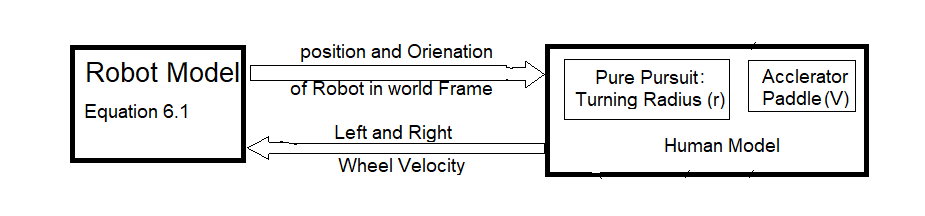
\includegraphics[width=\linewidth,keepaspectratio]{Chapter6/fig/SimulationModel}
	\captionof{figure}{Simulation scheme }
	\label{fig:SimBlock1} 
\end{figure}

  


\section{Simulation and Results }

The teleoperation loop consists of the operator model described in Section 6.2 at one end of the communication link and the mobile robot model described in Section 6.1 on the other end . As shown in Figure \ref{fig:teleloop}, there will a delay in both directions of communication. In real system, the video image is streamed  by the robot. Due to large quantity of data and limited bandwidth the delay $T_1>>T_2$. The amount of delay $h_1$ was experimentally measured  and it was found around 0.5 sec, as described in Appendix A. The command sent by the operator is  $v$ and $\dot{\theta}$ which is few bytes only.  Therefore in simulation  $h_2=0$ is assumed.


\begin{figure}
	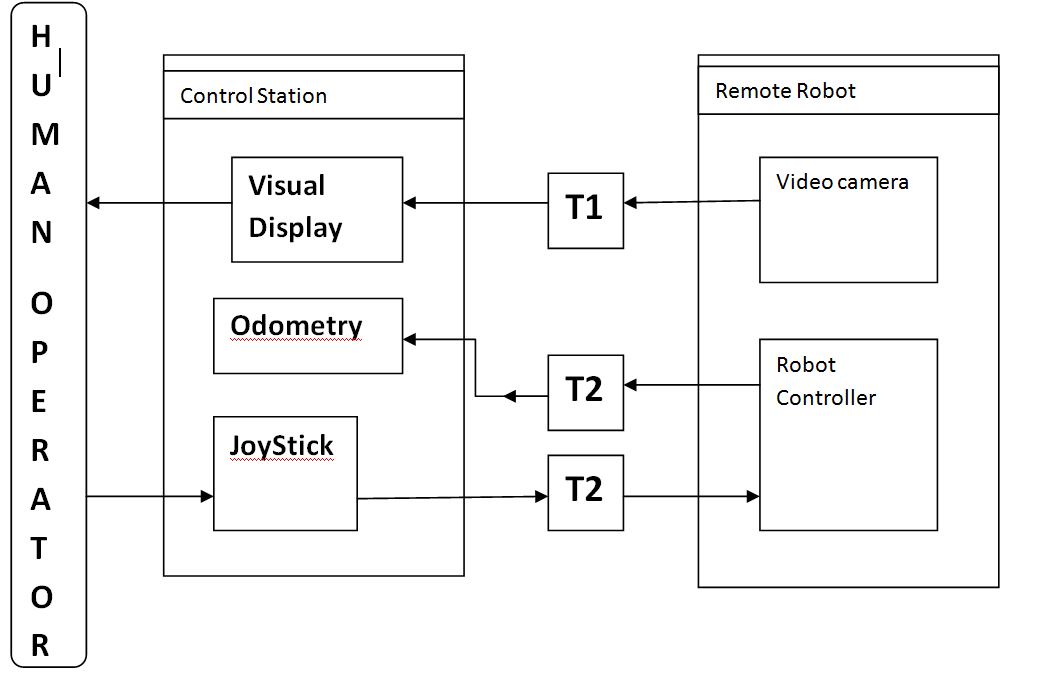
\includegraphics[width=\linewidth,keepaspectratio]{Chapter6/fig/BlockTimeDelay}
	\captionof{figure}{ Block diagram for teleoperation}
	\label{fig:teleloop} 
\end{figure}


\subsection{Simulation algorithm} 
The algorithm for simulation is explained in the following steps.
\begin{enumerate}
\item Convert the path from global coordinate system (CS) to Robots Local Coordinate System
\item With a given look ahead distance (l) search for a point on the path
\begin{itemize}
\item If point is found goto Step 3
\item If not found increase the look ahead distance 
\end{itemize}
\item Determine the turning radius (r) using Equation 6.5
\item Calculate the command to the robot based on Equation 6.6. Note that these commands are based on the old visual data the operator saw.
\item Solve delayed  differential equation.
\end{enumerate}

Simulation was carried using Matlab. Delay differential equation solver \textit{"dde24"} was used to solve Equations 6.1 and 6.2 with delayed inputs $u_r$ and $u_l$.  The desired path  was a circle of radius 5m centred at origin of the global coordinate system. The human action was modelled with look ahead distance of 0.5m and linear velocity of 0.5m/s. The initial position of the robot was (4.5,0.0).

 The  performance of the system with zero delay, i.e. $T_1=T_2=0$ is shown in Figure \ref{fig:nodelayplot}. Figures \ref{fig:delay500plot} and \ref{fig:delay800plot} show the   robot's motion under delay of 0.5 and 0.8 sec.  It is seen that oscillation becomes visible at 0.5sec delay, and with the delay of  0.8 sec the system was on the verge of instability. 
 
 It was also observed that the with large vehicle velocity, $v$ and large look ahead distance, $l$ the instability commences with smaller time delay, $\delta$ in Equation 6.2.  
\begin{figure}[h]
	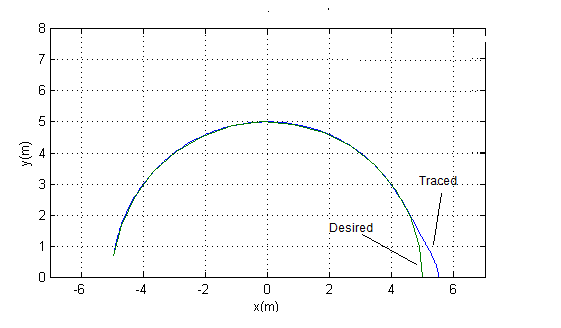
\includegraphics[width=\linewidth,keepaspectratio]{Chapter6/fig/noDelay}
	\captionof{figure}{Simulation with no time delay in either direction }
	\label{fig:nodelayplot} 
\end{figure} 
\begin{figure}[h]
	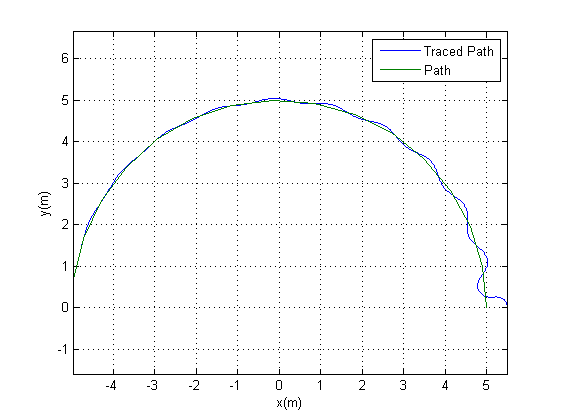
\includegraphics[width=\linewidth,keepaspectratio]{Chapter6/fig/Delay500milsec}
	\captionof{figure}{Simulation with  time delay $h_1=.5$ sec and $h_2=0$  sec }
	\label{fig:delay500plot} 
\end{figure} 
\begin{figure}[h]
	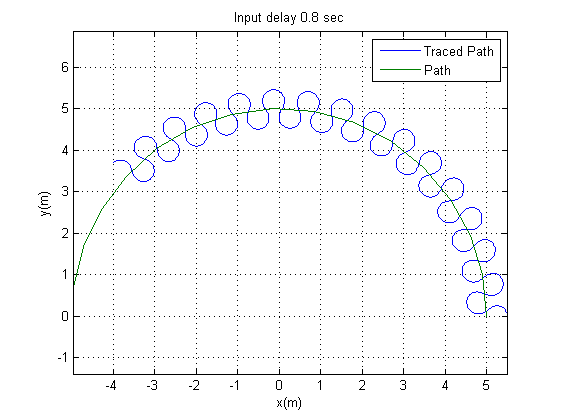
\includegraphics[width=\linewidth,keepaspectratio]{Chapter6/fig/Delay800milsec}
	\captionof{figure}{Simulation with  time delay $h_1=.8$ sec and $h_2=0$ sec }
	\label{fig:delay800plot} 
\end{figure} 

 In the next section we propose a predictive model based feedback control which is used to stabilize robot motion  under time delay teleopration.

\section{Summary}
In this chapter, simulation study of the developed teleoperated mobile robot is presented. A mathematical model of the action of human operator  while driving the robot based on visual feedback  was presented. Simulation results show that the behaviour of the system deteriorates with increase in delay in communication between the local and remote station. With large time delay the system becomes unstable.

